%
% $Id: $
%
%
% Compilar a .pdf con LaTeX (pdflatex)
% Es necesario instalar Beamer (paquete latex-beamer en Debian)
%

%
% Gr�ficos:
% Los gr�ficos pueden suministrarse en PNG, JPG, TIF, PDF, MPS
% Los EPS deben convertirse a PDF (usar epstopdf)
%

\documentclass{beamer}
\usetheme{Warsaw}
%\usebackgroundtemplate{
\includegraphics[width=\paperwidth]{format/libresoft-bg.png}}
%\usepackage[spanish]{babel}
\usepackage[latin1]{inputenc}
\usepackage{graphics}
\usepackage{amssymb} % Simbolos matematicos
\usepackage{url}

%\definecolor{libresoftgreen}{RGB}{162,190,43}
%\definecolor{libresoftblue}{RGB}{0,98,143}

%\setbeamercolor{titlelike}{bg=libresoftgreen}

%% Metadatos del PDF.
\hypersetup{
  pdftitle={Code to learn with Scratch? A systematic literature review},
  pdfauthor={J. Moreno-Le�n, Gregorio Robles},
  pdfcreator={GSyC/LibreSoft \\ Universidad Rey Juan Carlos},
  pdfproducer=PDFLaTeX,
  pdfsubject={Code to learn with Scratch},
}
%%

\begin{document}

\title{Code to learn with Scratch?}
\subtitle{A systematic literature review}
\institute{jesus.moreno@programamos.es, grex@gsyc.urjc.es \\
GSyC/Libresoft, Universidad Rey Juan Carlos}
\author{J. Moreno-Le�n, Gregorio Robles}
\date{IEEE EDUCON 2016, Abu Dhabi, April 12\textsuperscript{th} 2016}

\frame{
\maketitle
\begin{center}

\includegraphics[width=2cm]{format/libresoft-logo}
\hspace{0.5cm}

\includegraphics[width=5cm]{format/gsyc-urjc}
\vspace{0.5cm}

\includegraphics[width=3cm]{format/emadrid.png}
\end{center}
}


% Si el titulo o el autor se quieren acortar para los pies de p�gina
% se pueden redefinir aqu�:
%\title{Titulo corto}
%\author{Autores abreviado}

%% LICENCIA DE REDISTRIBUCION DE LAS TRANSPAS
\frame{
~
\vspace{3cm}

\begin{flushright}

\includegraphics[width=2.2cm]{figs/by-sa}

{\tiny
(cc) 2016 J. Moreno-Le�n and Gregorio Robles\\
  Some rights reserved. This work licensed under Creative Commons \\
  Attribution-ShareAlike License. To view a copy of full license, see \\
  http://creativecommons.org/licenses/by-sa/3.0/ or write to \\
  Creative Commons, 559 Nathan Abbott Way, Stanford, \\
  California 94305, USA. \\
\ \\
Some of the figures have been taken from the Internet \\
Source, and author and licence if known, is specified. \\
For those images, \emph{fair use} applies.
}
\end{flushright}
}
%%

\section{EDUCON 2016, Abu Dhabi}


%--------------------------------------------------------
%\usebackgroundtemplate{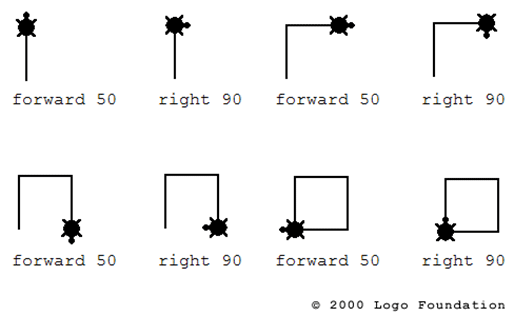
\includegraphics[height=10cm]{figs/turtles.png}}
% background: http://www.wim-network.org/wp-content/uploads/2012/04/iceberg.jpg

\begin{frame}
\frametitle{Code to learn (I)}
\begin{columns}[T]
  \begin{column}{0.5\textwidth}
    \begin{figure}[t!]
      \begin{center}
	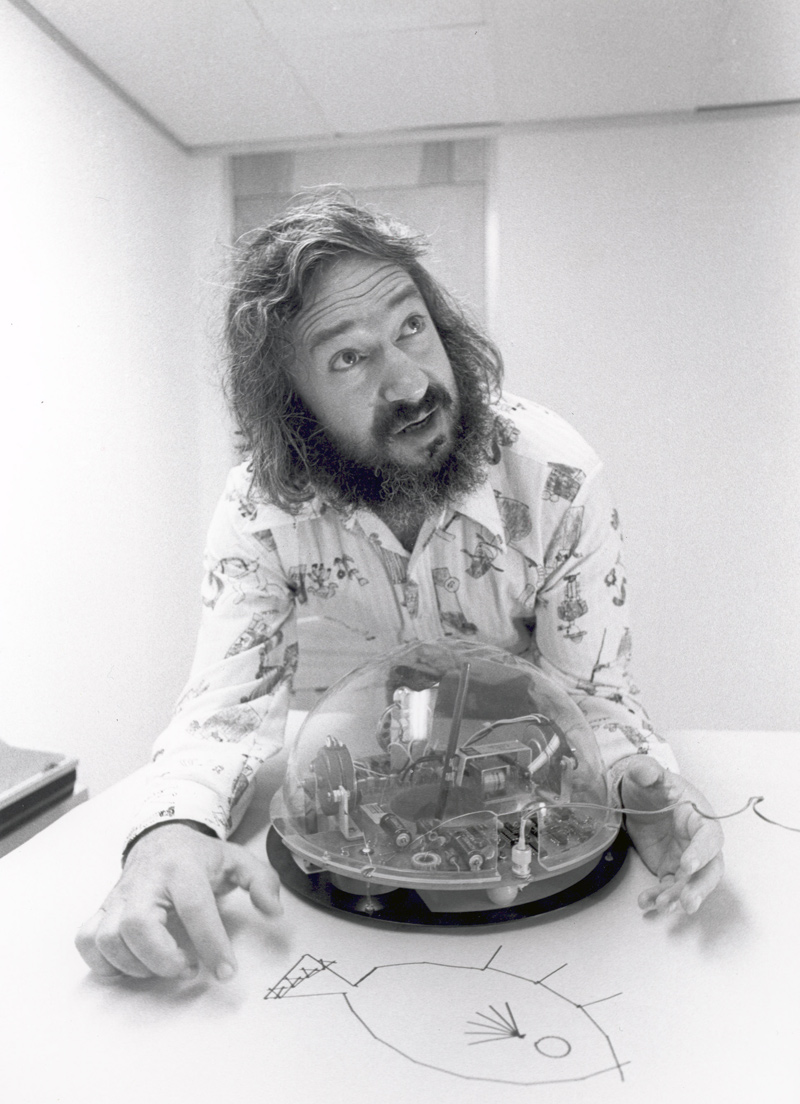
\includegraphics[width=5cm]{figs/seymour.jpg}
      \end{center}
      \label{fig:repetition1}
    \end{figure}
  \end{column}
  \begin{column}{0.5\textwidth}
    \begin{block}{Logo programming language}
      \begin{itemize}
	 \item Developed in the 1960s
         \item Its educational impact was intensively investigated in the 70s and 80s
         \item Students' improvements in maths (and other disciplines) were proved
         \item ``Disappeared'' from the educational landscape since mid-90s
      \end{itemize}
    \end{block}
    \hfill{\Tiny Seymour Papert's picture: jgora.net}
  \end{column}
\end{columns}
\end{frame}

\usebackgroundtemplate{}
%--------------------------------------------------------
\usebackgroundtemplate{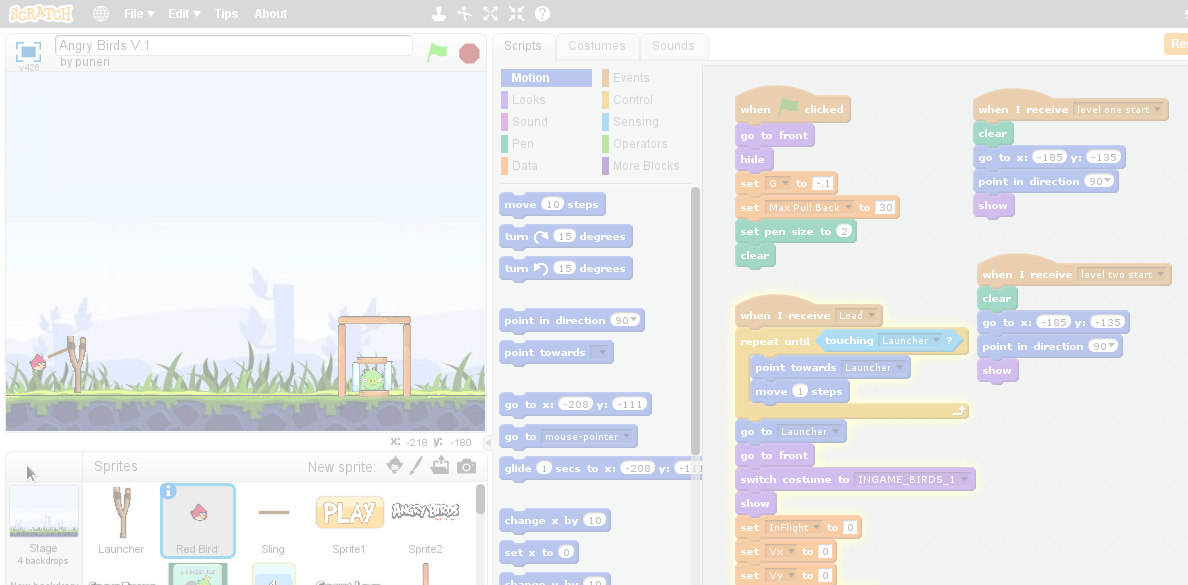
\includegraphics[width=18cm]{figs/AngryBirds2.png}}
\begin{frame}
\frametitle{Code to learn (and II)}

\begin{columns}[T]
  \begin{column}{1\textwidth}
     \begin{block}{New visual programming languages}
       \begin{itemize}
	 	 \item Alice, Greenfoot, Kodu, \textbf{Scratch}
         \item Code.org, EU Code Week, Africa Code Week, ArabCode.org 
         \item If there is no evidence showing educational impact of programming, this resurgence of programming in schools could disappear in a few years.
       \end{itemize}
    \end{block}
  \end{column}
\end{columns}

\end{frame}
\usebackgroundtemplate{}
%--------------------------------------------------------
\usebackgroundtemplate{
\includegraphics[width=14cm]{figs/goals.jpg}}
%https://rebel-performance.com/wp-content/uploads/2014/10/goals.jpg

\begin{frame}
\frametitle{Research questions}

\begin{itemize}
\item \Large  {\bf RQ1. What K-12 subjects have used programming with Scratch as an educational resource?}\\
\item \Large  {\bf RQ2. Is programming with Scratch a good educational tool that enhances student learning?}\\
\item \Large  {\bf RQ3. What other skills are developed while learning to code with Scratch?}
\end{itemize}
\hfill{\Tiny Background picture: rebel-performance.com}
\end{frame}

\usebackgroundtemplate{}
%-----------------------    ---------------------------------

\begin{frame}
\frametitle{Methodology}
\end{frame}

\usebackgroundtemplate{}

%-----------------------    ---------------------------------

\begin{frame}
\frametitle{Findings, RQ1}
\end{frame}

\usebackgroundtemplate{}

%-----------------------    ---------------------------------

\begin{frame}
\frametitle{Findings, RQ2}
\end{frame}

\usebackgroundtemplate{}

%-----------------------    ---------------------------------

\begin{frame}
\frametitle{Findings, RQ3}
\end{frame}

\usebackgroundtemplate{}

%-----------------------    ---------------------------------
%%\usebackgroundtemplate{
\includegraphics[width=13cm]{figs/take-away.jpg}}
%% background: http://2.bp.blogspot.com/-78Eh4TBpdtU/UPw7ULV73PI/AAAAAAAAHAE/6DQfvPNCo-Y/s1600/8723052-stylized-red-stamp-showing-the-term-take-away-all-on-white-background.jpg
\begin{frame}
\frametitle{Conclusions}
\end{frame}

\usebackgroundtemplate{}

%-----------------------    ---------------------------------
%\usebackgroundtemplate{
\includegraphics[width=14cm]{figs/audience.png}}
%% http://cdn.netrafic.com/wp-content/uploads/2011/02/audience.gif
%
%\begin{frame}
%\frametitle{Audience}
%
%Who should/could be interested in this talk?
%
%\begin{itemize}
%  \item Primary and Secondary teachers.
%  \item Language educators.
%  \item Students.
%  \item Developers of programming learning tools.
%\end{itemize} 
%
%\end{frame}
%
%\usebackgroundtemplate{}
%%--------------------------------------------------------
%\usebackgroundtemplate{\includegraphics[width=13cm,height=9.2cm]{figs/english.jpeg}}
%\begin{frame}
%\frametitle{English language skills of Spanish students}
%
%
%  \begin{columns}[T]
%    \begin{column}{1\textwidth}
%     \begin{block}{European Survey on Language Competences}
%\begin{itemize}
%  \item Assessed the English language skills of 53,000 secondary students from 14 countries
%  \item European Commission target: 50\% of students in CEFRL B1 or B2 level
%  \item Spanish results in 2014: just 30\%
%\end{itemize}
%    \end{block}
%    \end{column}
%    
%  \end{columns}
%\vspace{\baselineskip}
%\hfill{\Tiny Background picture: http://onesixstudio.com }
%\end{frame}
%
%\usebackgroundtemplate{}
%
%%--------------------------------------------------------
%\usebackgroundtemplate{\includegraphics[width=13cm,height=9.2cm]{figs/kids.jpeg}}
%\begin{frame}
%\frametitle{The study}
%
%
%  \begin{columns}[T]
%    \begin{column}{1\textwidth}
%     \begin{block}{Code to learn English with Scratch}
%\begin{itemize}
%  \item Quasi-Experimental Design
%  \item 65 students, 4\textsuperscript{th} and 5\textsuperscript{th} grades
%  \item Control groups and experimental groups
%  \item Pre and Post tests
%  \item Surveys
%\end{itemize}
%    \end{block}
%    \end{column}
%    
%  \end{columns}
%
%\end{frame}
%
%\usebackgroundtemplate{}
%
%%--------------------------------------------------------
%%\usebackgroundtemplate{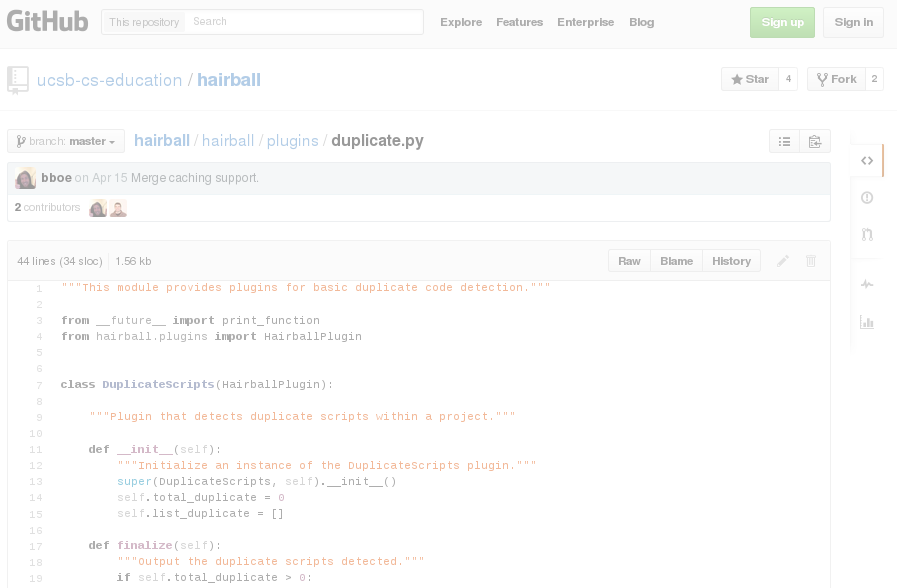
\includegraphics[width=13cm,height=9.2cm]{figs/plugins.png}}
%% background: http://25.media.tumblr.com/b83aa72682992ab34b8ce7e61c0cb7f9/tumblr_menxc7qcq61ryin08o1_r1_1280.jpg
%\begin{frame}
%\frametitle{Findings: Surveys}
%
%  \begin{columns}[T]
%    \begin{column}{0.5\textwidth}
%    \begin{figure}[t!]
%    
%      \includegraphics[width=5.6cm,height=4.5cm]{figs/survey1.png}
%    
%    \label{fig:repetition1}
%    \end{figure}
%Scratch helped me to learn English     
%    \end{column}
%    \begin{column}{0.5\textwidth}
%    \begin{figure}[t!]
%    
%      \includegraphics[width=5.6cm,height=4.5cm]{figs/survey2.png}
%    
%    \label{fig:repetition1}
%    \end{figure} 
%    Scratch made me want to learn more English
%    \end{column}
%  \end{columns}
%
%\end{frame}
%
%\usebackgroundtemplate{}
%
%%--------------------------------------------------------
%%\usebackgroundtemplate{\includegraphics[width=13cm]{figs/iceberg.jpg}}
%% background: http://www.wim-network.org/wp-content/uploads/2012/04/iceberg.jpg
%
%\begin{frame}
%\frametitle{Findings: English knowledge}
%
%\begin{table}
%\begin{center}
%  \begin{tabular}{ | l | c | c | }
%   \hline
%              & Experimental group & Control group \\ \hline\hline
%    Initial test & 5.05 & 5.13 \\ \hline
%    Final test & 7.7 & 7.55 \\ \hline
%    Improvement & 2.65 & 2.42 \\ \hline
%  \end{tabular}
%\end{center}
%\caption{Pre-test and Post-test results}
%\label{table:results}
%\end{table}
%\end{frame}
%
%%--------------------------------------------------------
%\begin{frame}
%\frametitle{Findings: Teacher training}
%
%  \begin{columns}[T]
%    \begin{column}{0.5\textwidth}
% 
%     \begin{block}{Experimental group 1}
%\begin{figure}[t!]
%\begin{center}
%\includegraphics[width=5.4cm,height=5.4cm]{figs/chart1.png}
%\end{center}
%Teacher with coding experiencie
%\label{fig:results1}
%\end{figure}
%     \end{block}
%    \end{column}
%    \begin{column}{0.5\textwidth}
%     \begin{block}{Experimental group 2}
%\begin{figure}[t!]
%\begin{center}
%\includegraphics[width=5.4cm,height=5.4cm]{figs/chart2.png}
%\end{center}
%First-time programmer teacher
%\label{fig:results2}
%\end{figure}
%     \end{block}
%
%    \end{column}
%  \end{columns}
%
%\end{frame}
%
%%--------------------------------------------------------
%\begin{frame}
%\frametitle{Findings: Coding skills}
%
%\begin{figure}[t!]
%\begin{center}
%\includegraphics[width=11cm, height=5.5cm]{figs/mastery.png}
%\end{center}
%\label{fig:naming}
%\end{figure}
%
%\begin{center}
%Computational Thinking Score - Dr. Scratch results 
%http://drscratch.programamos.es
%\end{center}
%\end{frame}
%
%%--------------------------------------------------------
%%\usebackgroundtemplate{
\includegraphics[width=13cm]{figs/take-away.jpg}}
%% background: http://2.bp.blogspot.com/-78Eh4TBpdtU/UPw7ULV73PI/AAAAAAAAHAE/6DQfvPNCo-Y/s1600/8723052-stylized-red-stamp-showing-the-term-take-away-all-on-white-background.jpg
\usebackgroundtemplate{
\includegraphics[width=13cm]{figs/future.png}}

\begin{frame}
\frametitle{Future Work}

%\begin{enumerate}
%  \item Increase the number of students
%  \item Increase the type of subjects 
%  \item Increase the working time of programming
%\end{enumerate}
%\vspace{\baselineskip}
%\vspace{\baselineskip}
%\hfill{\Tiny Background picture: Simon Cunningham }
%
\end{frame}
%
%%--------------------------------------------------------
%%\begin{frame}
%%\frametitle{GSyC/LibreSoft}
%
%%\begin{figure}[t!]
%%\begin{center}
%%\includegraphics[width=11cm]{figs/libresoft.jpg}
%%\end{center}
%%\label{fig:libresoft}
%%\end{figure}
%
%%\begin{center}
%%The GSyC/LibreSoft research team at URJC (Madrid).
%%\end{center}
%
%%\end{frame}
%
%%--------------------------------------------------------
%%\begin{frame}
%%\frametitle{Our work at GSyC/LibreSoft}
%
%%\begin{figure}[t!]
%%\begin{center}
%%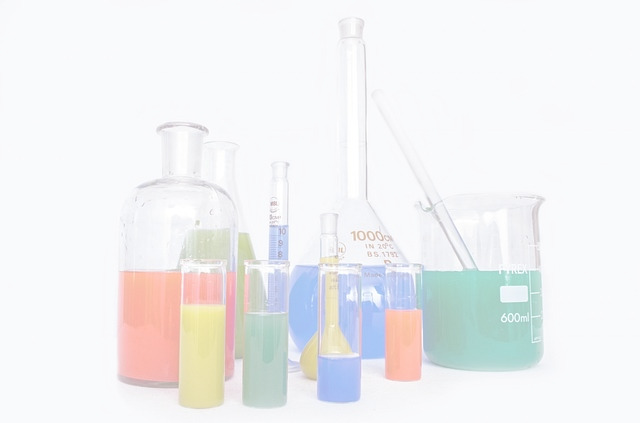
\includegraphics[width=2.5cm]{figs/research}
%% http://www.memphis.edu/crow/images/research_2.jpg
%%\hspace{0.1cm}
%%\includegraphics[width=2.5cm]{figs/teaching}
%% http://2.bp.blogspot.com/_uxgwfriLwSo/TOWDr8IjaLI/AAAAAAAABLM/d7H-G5jIq-c/s1600/teaching.gif
%%\hspace{0.1cm}
%%\includegraphics[width=2.5cm]{figs/development}
%% http://www.vidadigitalradio.com/wp-content/uploads/2009/04/hackers_cartoons.jpg
%%\hspace{0.1cm}
%%\includegraphics[width=2.5cm]{figs/promotion}
%% http://bloggeate.com/wp-content/uploads/2011/04/como-promocionar-tu-blog.jpg
%%\end{center}
%%\label{fig:whatwedo}
%%\end{figure}
%
%%\begin{center}
%%GSyC/LibreSoft's tasks: research, teaching, development, promotion of free software.
%
%%\end{center}
%%\end{frame}
%
\usebackgroundtemplate{}

%--------------------------------------------------------
\frame{
\maketitle
\begin{center}

\includegraphics[width=2cm]{format/libresoft-logo}
\hspace{0.5cm}

\includegraphics[width=5cm]{format/gsyc-urjc}
\vspace{0.5cm}

\includegraphics[width=3cm]{format/emadrid.png}
\end{center}
}

\end{document}
